\begin{frame}{Electric Power Consumption}


\bi
\mi One-minute-sampling of electric power consumption  
\begin{enumerate}
    \item in households
    \item over almost $4$ years
    \item total + three different categories 

  \end{enumerate}
\mi Electric Power Consumption
\mi $2,075,259\times9$
\mi $1.25\%$ missing values
\ei
\begin{columns}[t] % contents are top vertically aligned
     \begin{column}[T]{7cm} % each column can also be its own environment
     
     \end{column}
     \begin{column}[T]{5cm} % alternative top-align that's better for graphics
          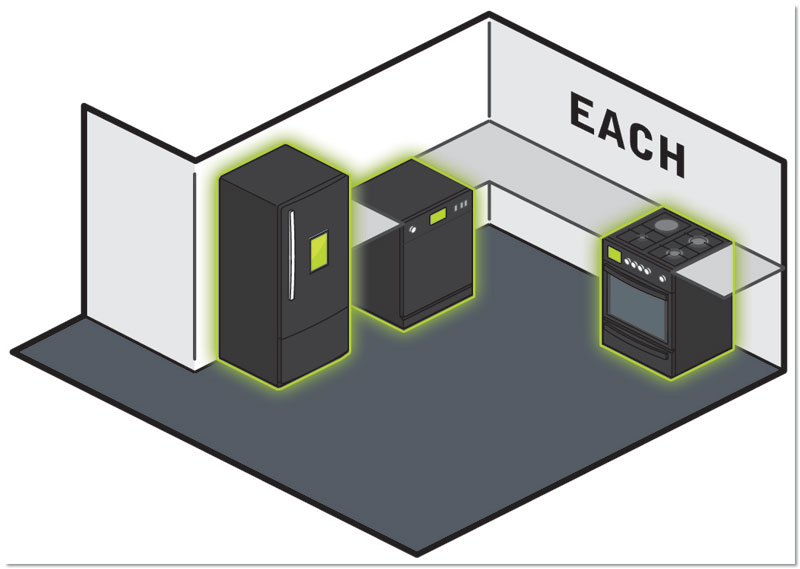
\includegraphics[height=3cm]{fig/each.jpg}
     \end{column}
 \end{columns}

\end{frame}

\begin{frame}{Electric Power Consumption}

\begin{tcolorbox}[colback=LightSteelBlue!5,colframe=yellow!40!black,title=Preprocessing]

\bi
\mi Date and Time
\begin{enumerate}
    \item Ticks {\tiny (100-nanosecond ticks since $\ldots$)}
    \item Epoch$_{Unix Time}$ {\tiny (Seconds since (UTC), Thursday, 1
    January 1970) }
  \end{enumerate}
\mi Normalisation/Scaling
\begin{enumerate}
<<<<<<< HEAD
    \item Standardization Scaling
=======
    \item Z-Score 
>>>>>>> 4036dffc4001522e9cb6425d34585080579db3cd
    \item MinMax 
  \end{enumerate}
  
  \mi Missing Values
\begin{enumerate}
    \item Three to one mapping 
    \item Eliminated
  \end{enumerate}
\ei


\end{tcolorbox}
\end{frame}

\begin{frame}{Electric Power Consumption}
\begin{tcolorbox}[colback=LightSteelBlue!5,colframe=yellow!40!black,title=Final
Comparison]


\begin{table}
\centering
\resizebox{\columnwidth}{!}
	{
		\begin{tabular}{|c|c|c|c|c|}
					\hline  &&& $1^{st}$ quartile
					&\\{Algorithm}&Mean&Standard Deviation&Median& Runtime (s)\\&&& $3^{rd}$
					quartile &\\
					\hline &&&$-3.19193$&\\
					{Linear Ridge
		Regression}& $0.05528$ & $6.70155$  & $-0.07853$ & $\bf {0.252}$\\
					 ($\alpha = 0.1$)&&&$1.97658$& \\
					\hline &&&$\bf {-0.50000}$&\\
					\bf {{$\mathbf {k-}$nearest neighbors}}& $\bf {0.02874}$ & $\bf {3.88777}$ 
					& $0.00000$ & $5.975$\\
					 ($k = 2$)&&&$\bf {0.50000}$& \\
					\hline &&&$-2.23407$&\\
					{Stochastic Gradient Descent }& $0.80390$ & $6.81799$  & $0.02416$ &
					$4.388$\\
					({\it huber}, $\epsilon = 0.1$ )&&&$1.93741$& \\
					\hline &&&$-$&\\
					{Support Vector Machine }& $-$ & $-$  & $-$ &
					$-$\\
					&&& $-$ & \\
					\hline

		\end{tabular}
	}



\end{table}



\end{tcolorbox}
\end{frame}

\begin{frame}{Electric Power Consumption}


\begin{tcolorbox}[colback=LightSteelBlue!5,colframe=yellow!40!black,title=Facts]

\bi
\mi Date and Time 
\begin{enumerate}
    \item $\mapsto$ Epoch
  \end{enumerate}
  
  \mi Normalisation/Scaling 
\begin{enumerate}
<<<<<<< HEAD
    \item Better results neither with MinMax nor Standardization Scaling 
=======
    \item Better results neither with MinMax nor Z-Score
>>>>>>> 4036dffc4001522e9cb6425d34585080579db3cd
  \end{enumerate}
 
\mi Selecting the best depends on expectations
  \mi Best results:
  \begin{itemize}
    \item Linear Ridge Regression $:$ Fastest
    \item $k$-Nearest Neighbors $:$ Most Accurate
  \end{itemize}
\ei


\end{tcolorbox}

\end{frame}
